\chapter{Theory}
%\label{chap:theory} this doesn't seem to work

%Theory relevant to the spectroscopy and detection of single Ba/Ba\textsuperscript{+} in SXe matrices is discussed.  Spectroscopy of Ba/Ba\textsuperscript{+} is first...

\section{Ba/Ba\textsuperscript{+} Spectroscopy in Vacuum}

The lowest-lying energy levels in vacuum for Ba and Ba\textsuperscript{+} are shown in Fig. \ref{fig:elevs}.  For Ba, the main transition is between the ground $6s^{2}$ $^{1}$S$_{0}$ to the excited $6s6p$ $^{1}$P$_{1}$ state.  Spin{\color{red}(?)}-suppressed transitions between the P state and three metastable D states results in a decay in to a D state after about 350 excitations.  For Ba\textsuperscript{+}, two strong transitions exist between the ground $6s$ $^{2}$S$_{1/2}$ and the $6p$ $^{2}$P$_{1/2}$ and $6p$ $^{2}$P$_{3/2}$ excited states.  Transitions to the two metastable D states are higher than for the atom, resulting in a decay into a D state after about 4 excitations.

\begin{figure}[H]
	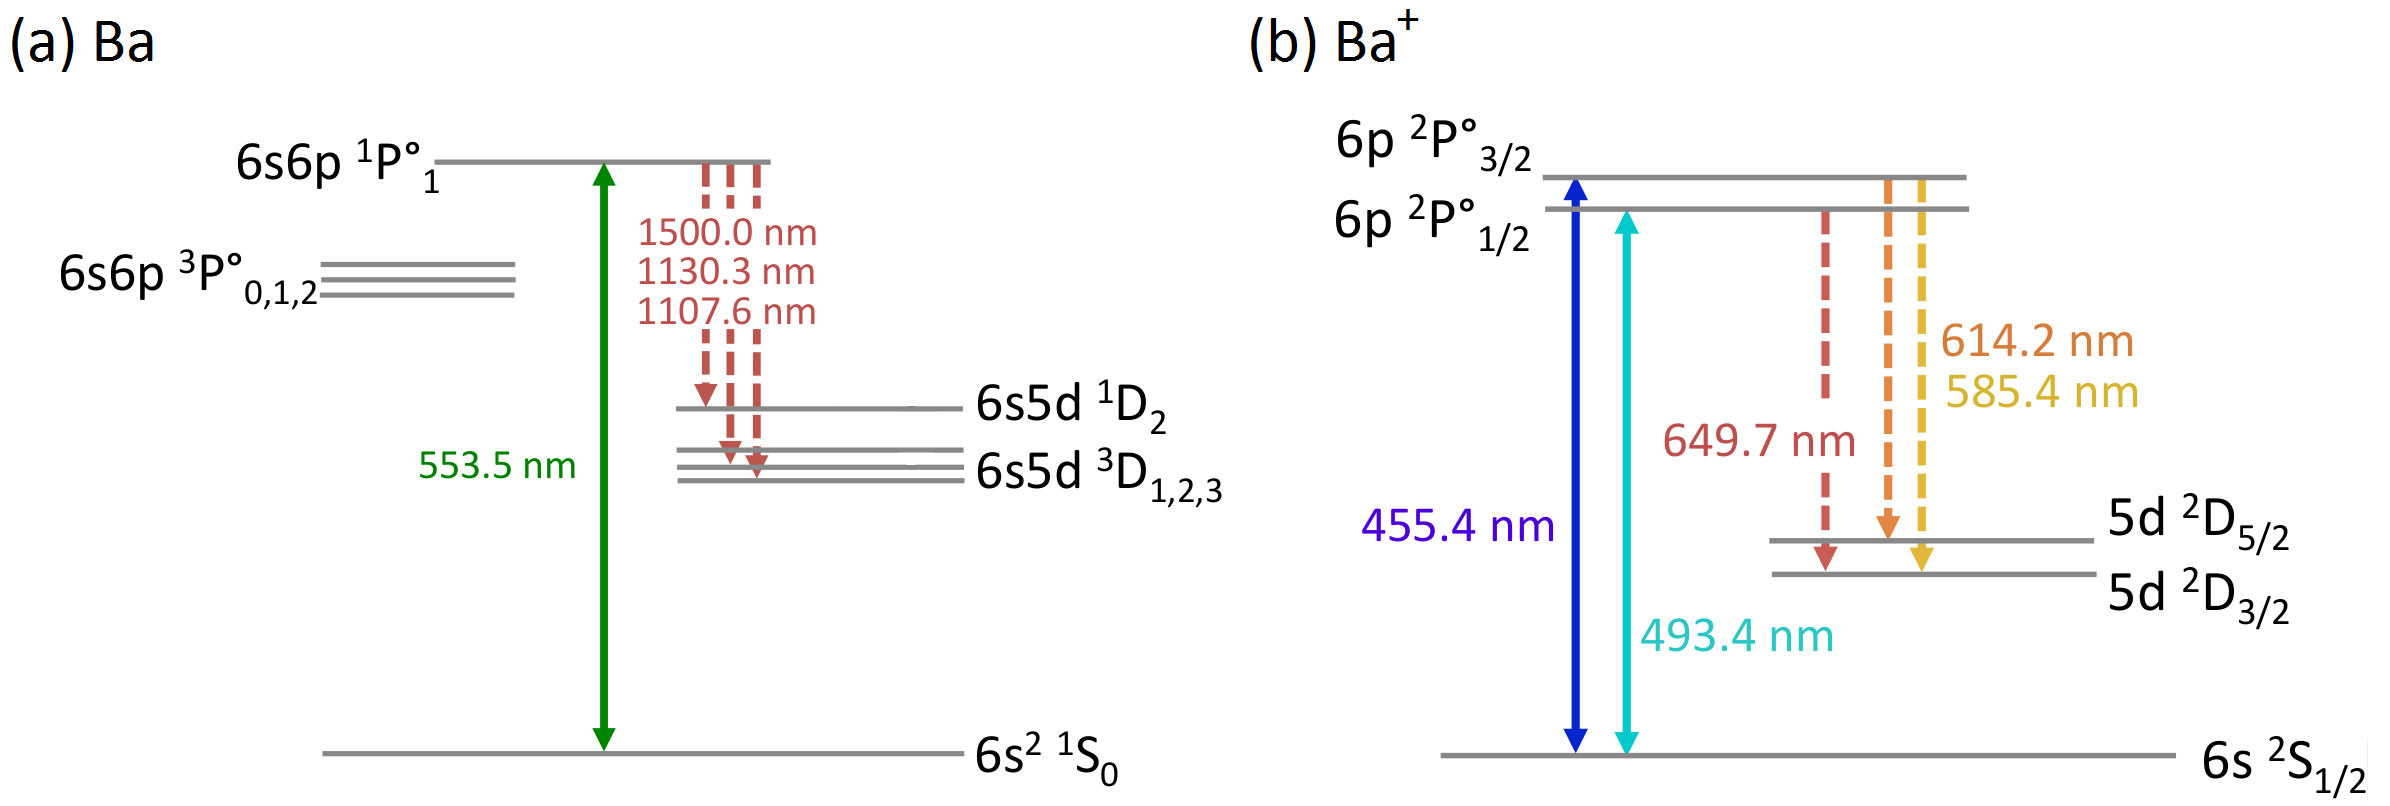
\includegraphics[width=.9\textwidth]{figures/elevs.png}
	\caption{Energy level diagrams for (a) Ba and (b) Ba\textsuperscript{+} ... \emph{\color{red}bah, you should have the blue AND the red Ba lines in there for reference from re-pumping section.}}
    \label{fig:elevs}
\end{figure}

These energy levels and their transition rates are well known, and are documented in the NIST Atomic Spectra Database.  Single atom/ion detection by spectroscopy generally requires, in addition to the main excitation laser, lasers to provide transitions out of the metastable D states once the atom/ion decays into one of them.  For the atom, this can be done via three additional infrared lasers for the direct transitions back to the $6s6p$ $^{1}$P$_{1}$ state, and also via excitation to higher-level states which have paths back to ground such as $6s6p$ $^{3}$D$_{1}$\textsuperscript{o}.  Trapping/detection of Ba atoms in a magneto-optical trap (MOT) is achieved in \cite{BaMOT}.  Single Ba\textsuperscript{+} observation requires only two lasers if the $^{2}$P$_{1/2}$ excited state is used.  This is demonstrated in [ref something that does this ... is there something?  How about the Carleton group?  I think MOE has a reference to it maybe -- yeah, its [19]].

\section{Matrix Isolation Spectroscopy}

%\emph{\color{gray}May be good matrix isolation theory references in Ba Spec... yeah, 1 and 2 i think ... shon's 55, 57, 58 are probably good too and maybe overlapping}

In the matrix isolation spectroscopy technique \emph{\color{gray}ref the original paper or whatev... maybe Crepin's [9] if different from Shons's}, the species of interest, e.g. Ba/Ba\textsuperscript{+}, is embedded and trapped in an inert host matrix, e.g. solid Xe, ideally with a host:guest ratio of $10^{3}$ or greater for a low probability of guest-guest interaction.  The ground S state of Ba, as well as for Ba\textsuperscript{+}, is spherically symmetric, and being slightly larger in Van der Waals radius than Xe, it is likely to take the place of one or more Xe atoms in the fcc crystal (substitution), vs. existing in between Xe atoms in the crystal structure (interstitial).  However, the strength of the Ba-Xe interaction, an induced dipole-dipole Van der Waals force, is likely quite different when the Ba is in the non-spherically-symmetric excited P state [crepin].  This leads to significant broadening of absorption and emission for the Ba, as well as an energy shift between the two, according to the Franck Condon Principle, illustrated in Fig. [fig franck condon].  In a cold matrix, the system will be in the ground lattice vibrational state before excitation.  Electronic excitation can occur to multiple vibrational modes whose wavefunctions overlap that of the ground state, thus broadening the absorption energy.  In the excited state, rapid decay occurs to the lowest vibrational mode before electronic decay can occur \emph{\color{gray}ref?} and then a similar broadening in the spontaneous emission energy occurs.  A redshift in the emission is observed relative to the excitation.

%\emph{\color{gray}Jahn-Teller?}

\emph{\color{gray}Talk about Ba in Ar?} {\color{red}[look at paper]}

Energy level transition probabilities can also be affected in a matrix, e.g., spin-fobidden transitions can become more significant via the heavy atom effect [crepin].  If electronic potential energy curves cross each other, non-radiative transitions can become allowed for otherwise forbidden transitions [crepin?].  Effects like these could aid in observation of the Ba/Ba\textsuperscript{+}, e.g. by improving decay rates out of metastable D states, or they could reduce detectability, e.g. if a non-radiative decay competes with the fluorescence channel.

%The detectability of a single atom/ion can depend greatly on [these]...

\section{6-level System}

Neutral Ba in vacuum is a 5-level system.  However, solving a 6-level system is helpful in modeling matrix-isolated Ba, where another state could be reached after excitation, e.g. decay into a \textsuperscript{3}P state.  The set of rate equations for this system is shown in Eqn. \ref{eqn:rateEqn}:

\begin{equation}
\begin{aligned}
\frac{dN_1}{dt} &= - w_{12}N_{1} + a_{21}N_{2} + a_{31}N_{3} + a_{41}N_{4} + a_{51} N_{5} + a_{61}N_{6} \\
\frac{dN_2}{dt} &= w_{12}N_{1} - N_{2}(a_{21} + a_{23} + a_{24} + a_{25} + a_{26}) \\
\frac{dN_3}{dt} &= a_{23}N_{2} - a_{31}N_{3} \\
\frac{dN_4}{dt} &= a_{24}N_{2} - a_{41}N_{4} \\
\frac{dN_5}{dt} &= a_{25}N_{2} - a_{51}N_{5} \\
\frac{dN_6}{dt} &= a_{26}N_{2} - a_{61}N_{6}
\end{aligned}
\label{eqn:rateEqn}
\end{equation}

\section{Fluorescence Efficiency}

Fluorescence efficiency, $\epsilon_{f}$, is the ratio of fluorescence photons emitted to excitations to the fluorescing state.  This becomes less than one when there are paths out of the excited state other than the one which emits the photon being measured, e.g. the $\epsilon_{f}$ of Ba in vacuum is about 99.7\%, not quite 1 due to about 1 in 350 decays from the P state into a metastable D state rather than back to ground.  $\epsilon_{f}$ can be calculated by Eqn. \ref{eqn:flueEff}:

\begin{equation}
\epsilon_{f} = \frac{f}{w_{12} \epsilon_{c}} = {\color{red}\frac{f h \nu}{\sigma I \epsilon_{c}}}
\label{eqn:flueEff}
\end{equation}

\noindent
where $f$ is the number of fluorescence photons observed, $w_{12}$ is the excitation rate, $\epsilon_{c}$ is the collection efficiency of the system, $\sigma$ is the cross section for the excitation interaction, $I$ is the laser intensity, and $h \nu$ is the excitation photon energy.  $\sigma$ can be measured by experiment, and the remaining parameters are easily calculated to produce a measurement of $\epsilon_{f}$.